\documentclass{article}
\usepackage[T1]{fontenc}
\usepackage[utf8]{inputenc}
\usepackage[polish]{babel}
\usepackage{amsmath}
\usepackage{multirow}
\usepackage{listings}
\usepackage{listingsutf8}
\usepackage{longtable}
\usepackage{float}
\usepackage{graphicx}
\usepackage{caption}
%{Informatyka stosowana 2020, I st., semestr VI}


\author{
	{Kacper Czernik 242371} \\
	{Mateusz Grzeszczak 242398}\\
{Prowadzący: Dr inż. Marcin Kacprowicz }
}

\title{Komputerowe systemy rozpoznawania 2020/2021\\Projekt 2. Podsumowania lingwistyczne relacyjnych baz danych}
\begin{document}
\maketitle

\section{Cel}
W ramach projektu zaimplementowano aplikację umożliwiającą lingwistyczną agregację danych liczbowych z wykorzystaniem logiki rozmytej. Poprzez stworzenie struktury klas reprezentujących różne typy zbiorów rozmytych oraz operacje na nich, aplikacja generuje podsumowania lingwistyczne w języku quasi-naturalnym \cite{zadrozny06}. Dzięki interfejsowi graficznemu użytkownicy mogą dostosować generowane podsumowania poprzez wybór predefiniowanych sumaryzatorów, kwalifikatorów i kwantyfikatorów, określanie wag dla miar jakości oraz sortowanie wyników.\\

\section{Baza danych, zmienne lingwistyczne, kwantyfikatory lingwistyczne}

\subsection{Charakterystyka podsumowywanej bazy danych}

W ramach projektu wybrano bazę danych \cite{dataBase}, zawierającą pomiary parametrów zbiorników wodnych wokół Irlandii. Baza ta zawiera łącznie 281 600 rekordów, jednak po wykluczeniu wartości "Null"  pozostaje ponad 210 tysięcy wyników. Zestaw danych posiada 12 kolumn możliwych do rozmycia, z których 4 zostaną połączone podczas pre-procesingu danych, w celu zachowania logicznej spójności podsumowania. Przykładowe wartości dla tego zbioru danych przedstawiono poniżej (Tabela 1). Kolumny latitude\_degrees\_north oraz longitude\_degrees\_east zostaną połączone, aby reprezentować odległość od środka Irlandii, umożliwiając identyfikację położenia pomiaru w zależności od części kraju. Analogicznie, kolumny sea\_surface\_x\_velocity\_m\_s oraz \\sea\_surface\_y\_velocity\_m\_s zostaną połączone w celu reprezentacji bezwzględnej prędkości wody, ułatwiając podsumowywanie wyników.

\begin{figure}[H]
\centering
\includegraphics[width=1\textwidth]{assets/dataBase.png}
\caption{Marine Institute Monthly Model Means $\epsilon$}
\label{fig:epsilon_bat}
\end{figure}


\subsection{Zmienne lingwistyczne (atrybuty/własności obiektów)}

W ramach projektu opisano zmienne lingwistyczne, nadając im etykiety oraz prezentując wykresy funkcji przynależności oraz wzory analityczne. Poniżej przedstawiono opisy poszczególnych zmiennych wraz z ich definicjami:

\subsubsection{Miejsce pomiaru}

Najbardziej niestandardową zmienną lingwistyczną utworzoną na potrzeby zadania jest miejsce pobierania pomiaru, zmienna ta składać się będzie z dwóch części: szerokości geograficznej oraz długości geograficznej. Dla obu tych części utworzone zostały osobne funkcje przynależności pozwalające na dokładne opisanie miejsca, w którym dany pomiar został zebrany. \\

Poniżej znajduje się mapa na której zaznaczony został obszar poddany badaniom.

\begin{figure}[H]
\centering
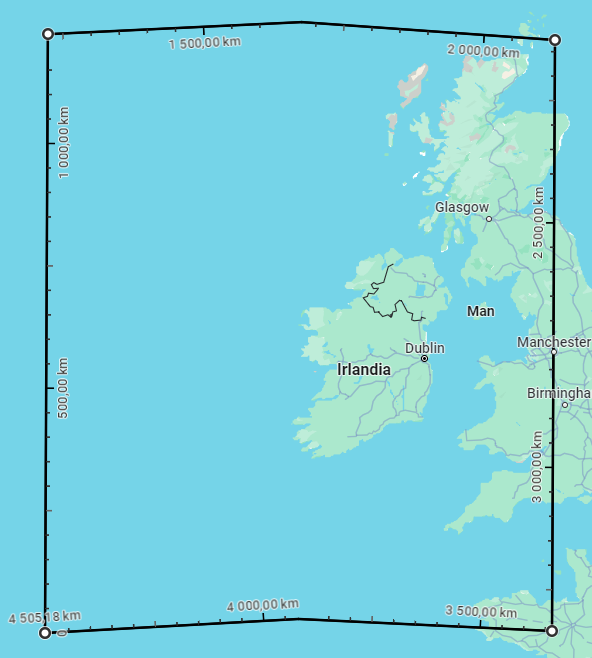
\includegraphics[scale=0.2]{ksr/projekt_2_fuzzy/assets/map.png}
\label{fig:epsilon_bat}
\end{figure}

\begin{equation*}
\begin{minipage}{0.5\textwidth}
\centering
\text{\scalebox{0.5}{na zachód od Irlandii}}(x) = \scalebox{0.5}{$
\begin{cases}
1 & \text{dla } x \leq -10.5 \\
\frac{-9 - x}{1.5} & \text{dla } -10.5 < x \leq -9 \\
0 & \text{w przeciwnym przypadku}
\end{cases}
$}
\end{minipage}%
\begin{minipage}{0.5\textwidth}
\centering
\text{\scalebox{0.5}{na południe od Irlandii}}(x) = \scalebox{0.5}{$
\begin{cases}
1 & \text{dla } x \leq 51.5 \\
\frac{52 - x}{0.5} & \text{dla } 51.5 < x \leq 52 \\
0 & \text{w przeciwnym przypadku}
\end{cases}
$}
\end{minipage}
\end{equation*}
\begin{equation*}
\begin{minipage}{0.5\textwidth}
\centering
\text{\scalebox{0.5}{na szerokości Irlandii}}(x) = \scalebox{0.5}{$
\begin{cases}
\frac{x - (-10.5)}{1.5} & \text{dla } -10.5 < x \leq -9 \\
1 & \text{dla } -10.5 < x < -6.3 \\
\frac{-5.4 - x}{0.9} & \text{dla } -6.3 < x \leq -5.4 \\
0 & \text{w przeciwnym przypadku}
\end{cases}
$}
\end{minipage}%
\begin{minipage}{0.5\textwidth}
\centering
\text{\scalebox{0.5}{na szerokości Irlandii}}(x) = \scalebox{0.5}{$
\begin{cases}
\frac{x - 51.5}{0.5} & \text{dla } 51.5 < x \leq 52 \\
1 & \text{dla } 52 < x < 55 \\
56 - x & \text{dla } 55 < x \leq 56 \\
0 & \text{w przeciwnym przypadku}
\end{cases}
$}
\end{minipage}
\end{equation*}
\begin{equation*}
\begin{minipage}{0.5\textwidth}
\centering
\text{\scalebox{0.5}{na wschód od Irlandii}}(x) = \scalebox{0.5}{$
\begin{cases}
0 & \text{dla } x \leq -6.3 \\
\frac{x - (-6.3)}{0.9} & \text{dla } -6.3 < x \leq -5.4 \\
1 & \text{w przeciwnym przypadku}
\end{cases}
$}
\end{minipage}%
\begin{minipage}{0.5\textwidth}
\centering
\text{\scalebox{0.5}{na północ od Irlandii}}(x) = \scalebox{0.5}{$
\begin{cases}
0 & \text{dla } x \leq 55 \\
x - 55 & \text{dla } 55 < x \leq 56 \\
1 & \text{w przeciwnym przypadku}
\end{cases}
$}
\end{minipage}
\end{equation*}




\begin{table}[H]
\centering
\begin{tabular}{cc}
    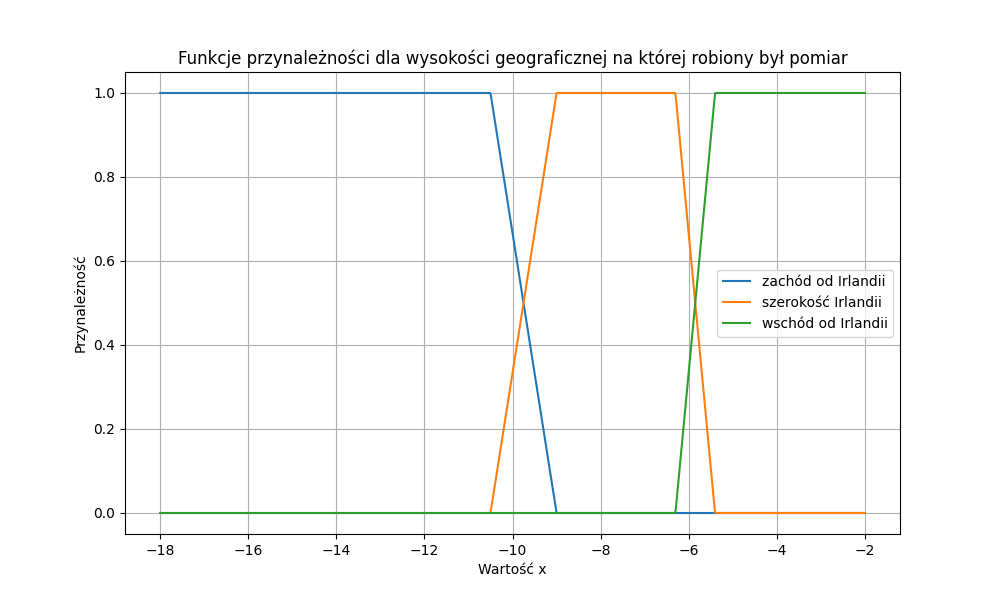
\includegraphics[width=0.5\textwidth]{ksr/projekt_2_fuzzy/assets/longitude.png} &
    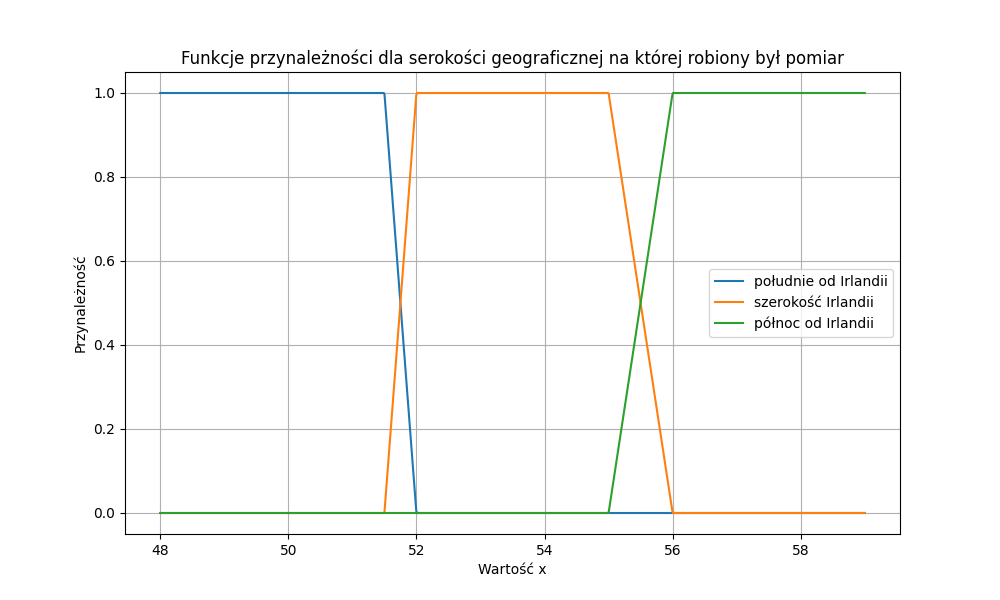
\includegraphics[width=0.5\textwidth]{ksr/projekt_2_fuzzy/assets/latitude.png} \\
     \\
\end{tabular}
\label{fig:two_images}
\end{table}

%===================================================================================================
\subsubsection{Temperatura na powierzchni}

\noindent Poniżej zaprezentowany został podział temperatury na wyselekcjonowane etykiety wraz z funkcjami przynależności dla każdej z nich. Zmienna ta opisuje temperaturę uzyskaną podczas pomiaru na powierzchni tafli wody.

\begin{equation*}
\begin{minipage}{0.5\textwidth}
\centering
\text{\scalebox{0.5}{zimna}}(x) = \scalebox{0.5}{$
\begin{cases}
1 & \text{dla } x \leq 12.5 \\
\frac{14 - x}{1.5} & \text{dla } 12.5 < x \leq 14 \\
0 & \text{w przeciwnym przypadku}
\end{cases}
$}
\end{minipage}%
\begin{minipage}{0.5\textwidth}
\centering
\text{\scalebox{0.5}{umiarkowana}}(x) = \scalebox{0.5}{$
\begin{cases}
\frac{x - 15.5}{1.5} & \text{dla } 15.5 < x < 17 \\
1 & \text{dla } x = 17 \\
\frac{18.5 - x}{1.5} & \text{dla } 17 < x \leq 18.5 \\
0 & \text{w przeciwnym przypadku}
\end{cases}
$}
\end{minipage}
\end{equation*}
\begin{equation*}
\begin{minipage}{0.5\textwidth}
\centering
\text{\scalebox{0.5}{chłodna}}(x) = \scalebox{0.5}{$
\begin{cases}
\frac{x - 13}{1.5} & \text{dla } 13 < x < 14.5 \\
1 & \text{dla } x = 14.5 \\
\frac{16.5 - x}{2} & \text{dla } 14.5 < x \leq 16.5 \\
0 & \text{w przeciwnym przypadku}
\end{cases}
$}
\end{minipage}%
\begin{minipage}{0.5\textwidth}
\centering
\text{\scalebox{0.5}{ciepła}}(x) = \scalebox{0.5}{$
\begin{cases}
0 & \text{dla } x \leq 18 \\
\frac{x - 18}{1.5} & \text{dla } 18 < x \leq 19.5 \\
1 & \text{w przeciwnym przypadku}
\end{cases}
$}
\end{minipage}
\end{equation*}




\begin{figure}[H]
\centering
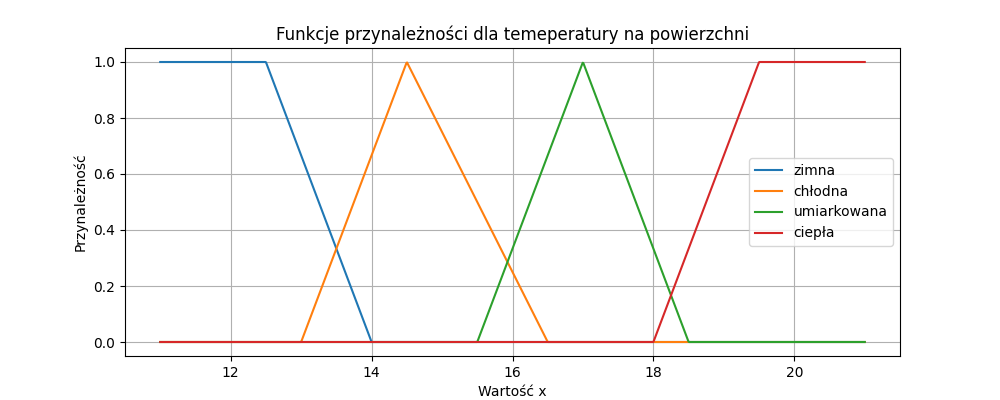
\includegraphics[width=0.5\textwidth]{ksr/projekt_2_fuzzy/assets/tmp_surface.png}
\label{fig:epsilon_bat}
\end{figure}

%===================================================================================================
\subsubsection{Temperatura na dnie}

\noindent Zmienna ta działa podobnie jak zmienna opisująca temperaturę na powierzchni z tą różnicą, że opisuje temperaturę zmierzoną na dnie zbiornika wodnego. Poniżej znajdują się wzory przynależności dla tej zmiennej lingwistycznej.

\begin{equation*}
\begin{minipage}{0.5\textwidth}
\centering
$\text{\scalebox{0.5}{zimna}}(x) =
\scalebox{0.5}{$
\begin{cases}
1 & \text{dla } x \leq 3 \\
\frac{5 - x}{2} & \text{dla } 3 < x \leq 5 \\
0 & \text{w przeciwnym przypadku}
\end{cases}
$}$
\end{minipage}%
\begin{minipage}{0.5\textwidth}
\centering
$\text{\scalebox{0.5}{umiarkowana}}(x) =
\scalebox{0.5}{$
\begin{cases}
\frac{x - 8}{2} & \text{dla } 8 < x \leq 10 \\
1 & \text{dla } 10 < x \leq 11 \\
\frac{13 - x}{2} & \text{dla } 11 < x \leq 13 \\
0 & \text{w przeciwnym przypadku}
\end{cases}
$}$
\end{minipage}
\end{equation*}

\begin{equation*}
\begin{minipage}{0.5\textwidth}
\centering
$\text{\scalebox{0.5}{chłodna}}(x) =
\scalebox{0.5}{$
\begin{cases}
\frac{x - 3}{3} & \text{dla } 3 < x \leq 6 \\
1 & \text{dla } 6 < x \leq 8 \\
9 - x & \text{dla } 8 < x \leq 9 \\
0 & \text{w przeciwnym przypadku}
\end{cases}
$}$
\end{minipage}%
\begin{minipage}{0.5\textwidth}
\centering
$\text{\scalebox{0.5}{ciepła}}(x) =
\scalebox{0.5}{$
\begin{cases}
x - 12 & \text{dla } 12 < x \leq 13 \\
1 & \text{dla } 13 < x \leq 14 \\
\frac{17 - x}{3} & \text{dla } 14 < x \leq 17 \\
0 & \text{w przeciwnym przypadku}
\end{cases}
$}$
\end{minipage}
\end{equation*}

\begin{equation*}
\begin{minipage}{0.5\textwidth}
\centering
$\text{\scalebox{0.5}{bardzo ciepła}}(x) =
\scalebox{0.5}{$
\begin{cases}
\frac{x - 15.5}{1.5} & \text{dla } 15.5 < x < 17 \\
1 & \text{dla } x = 17 \\
18 - x & \text{dla } 17 < x \leq 18 \\
0 & \text{w przeciwnym przypadku}
\end{cases}
$}$
\end{minipage}%
\begin{minipage}{0.5\textwidth}
\centering
$\text{\scalebox{0.5}{skrajnie ciepła}}(x) =
\scalebox{0.5}{$
\begin{cases}
0 & \text{dla } x \leq 17.5 \\
x - 17.5 & \text{dla } 17.5 < x \leq 18.5 \\
1 & \text{w przeciwnym przypadku}
\end{cases}
$}$
\end{minipage}
\end{equation*}



\begin{figure}[H]
\centering
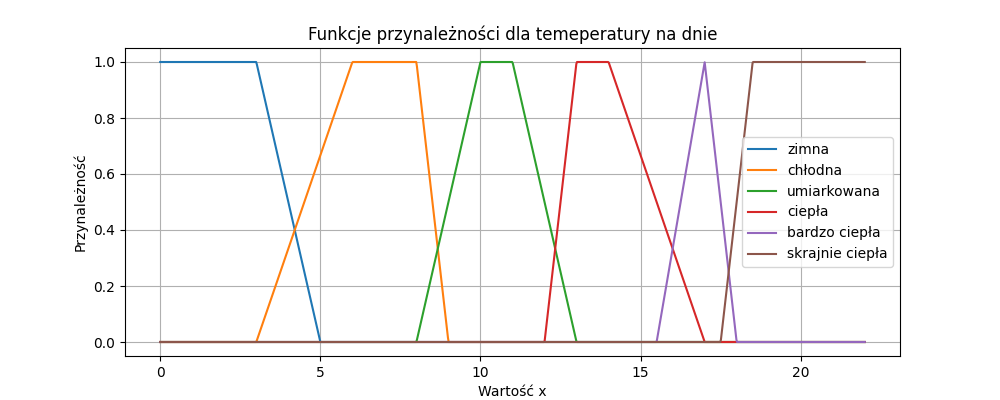
\includegraphics[width=0.5\textwidth]{ksr/projekt_2_fuzzy/assets/tmp_bottom.png}
\label{fig:epsilon_bat}
\end{figure}

%===================================================================================================
\subsubsection{Zasolenie na powierzchni}

\noindent Zmienna lingwistyczna opisująca zasolenie na powierzchni tafli wody, wartości przedstawione są w jednostkach zasolenia [PSU].

\begin{equation*}
\text{\scalebox{0.5}{umiarkowanie słona}}(x) =
\scalebox{0.5}{$
\begin{cases}
1 & \text{dla } x \leq 26 \\
\frac{30 - x}{4} & \text{dla } 26 < x \leq 30 \\
0 & \text{w przeciwnym przypadku}
\end{cases}
$}
\end{equation*}

\begin{equation*}
\text{\scalebox{0.5}{silnie słona}}(x) =
\scalebox{0.5}{$
\begin{cases}
\frac{x - 26}{4} & \text{dla } 26 < x \leq 30 \\
1 & \text{dla } 30 < x < 33 \\
\frac{35 - x}{2} & \text{dla } 33 < x \leq 35 \\
0 & \text{w przeciwnym przypadku}
\end{cases}
$}
\end{equation*}

\begin{equation*}
\text{\scalebox{0.5}{bardzo silnie słona}}(x) =
\scalebox{0.5}{$
\begin{cases}
0 & \text{dla } x \leq 34 \\
x - 34 & \text{dla } 34 < x \leq 35 \\
1 & \text{w przeciwnym przypadku}
\end{cases}
$}
\end{equation*}


\begin{figure}[H]
\centering
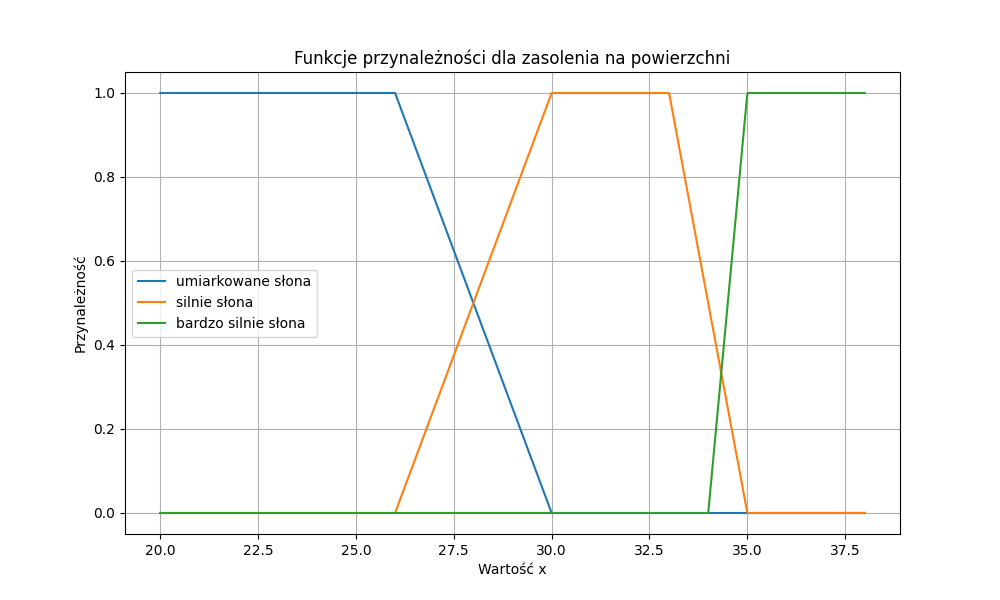
\includegraphics[width=0.5\textwidth]{ksr/projekt_2_fuzzy/assets/salinity_surface.png}
\label{fig:epsilon_bat}
\end{figure}

%===================================================================================================
\subsubsection{Zasolenie na dnie}

\noindent Ta zmienna lingwistyczna opisuje zasolenie na dnie opisane w jednostkach zasolenia [PSU].

\begin{equation*}
\begin{minipage}{0.5\textwidth}
\centering
\text{\scalebox{0.5}{nie słona}}(x) = \scalebox{0.5}{$
\begin{cases}
1 & \text{dla } x \leq 22 \\
\frac{26 - x}{4} & \text{dla } 22 < x \leq 26 \\
0 & \text{w przeciwnym przypadku}
\end{cases}
$}
\end{minipage}%
\begin{minipage}{0.5\textwidth}
\centering
\text{\scalebox{0.5}{umiarkowanie słona}}(x) = \scalebox{0.5}{$
\begin{cases}
\frac{x - 24}{2} & \text{dla } 24 < x \leq 26 \\
1 & \text{dla } 26 < x \leq 30.5 \\
\frac{32 - x}{1.5} & \text{dla } 30.5 < x \leq 32 \\
0 & \text{w przeciwnym przypadku}
\end{cases}
$}
\end{minipage}
\end{equation*}

\begin{equation*}
\begin{minipage}{0.5\textwidth}
\centering
\text{\scalebox{0.5}{silnie słona}}(x) = \scalebox{0.5}{$
\begin{cases}
\frac{x - 30.5}{3.5} & \text{dla } 30.5 < x < 34 \\
1 & \text{dla } x = 34 \\
\frac{36 - x}{2} & \text{dla } 34 < x \leq 36 \\
0 & \text{w przeciwnym przypadku}
\end{cases}
$}
\end{minipage}%
\begin{minipage}{0.5\textwidth}
\centering
\text{\scalebox{0.5}{bardzo silnie słona}}(x) = \scalebox{0.5}{$
\begin{cases}
0 & \text{dla } x \leq 35 \\
x - 35 & \text{dla } 35 < x \leq 36 \\
1 & \text{w przeciwnym przypadku}
\end{cases}
$}
\end{minipage}
\end{equation*}



\begin{figure}[H]
\centering
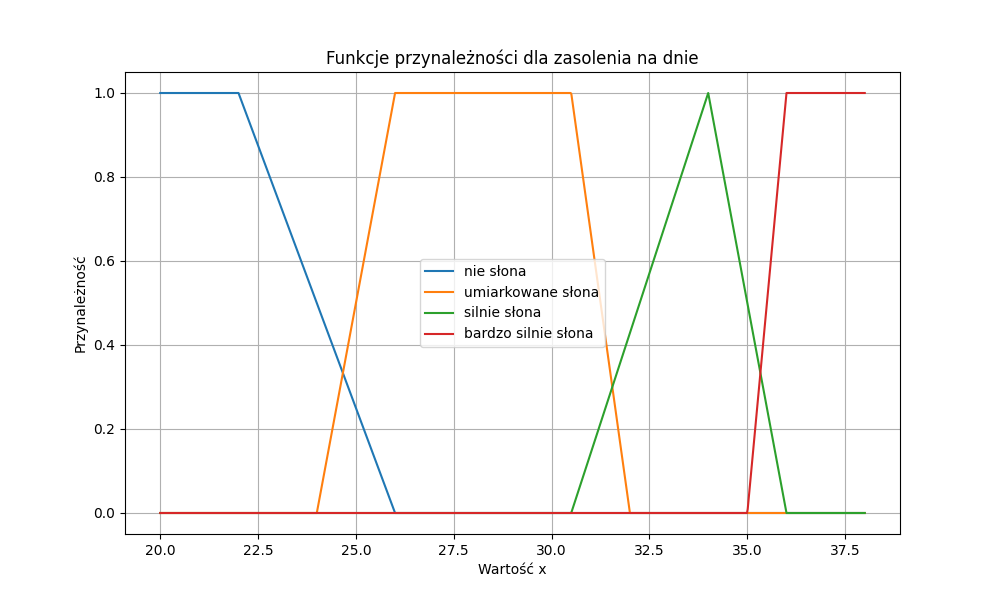
\includegraphics[width=0.5\textwidth]{ksr/projekt_2_fuzzy/assets/salinity_bottom.png}
\label{fig:epsilon_bat}
\end{figure}

%===================================================================================================
\subsubsection{Prędkość wody}

\noindent Wspomniana Zmienna opisuje prędkość, z jaką poruszała się woda w miejscu pomiaru w momencie jego robienia, jednostka, w której dane zostały zebrane to [m/s].

\begin{equation*}
\begin{minipage}{0.5\textwidth}
\centering
$\text{\scalebox{0.5}{praktycznie bez prędkości}}(x) =
\scalebox{0.5}{$
\begin{cases}
1 & \text{dla } x \leq 0.05 \\
\frac{0.1 - x}{0.05} & \text{dla } 0.05 < x \leq 0.1 \\
0 & \text{w przeciwnym przypadku}
\end{cases}
$}$
\end{minipage}%
\begin{minipage}{0.5\textwidth}
\centering
$\text{\scalebox{0.5}{bardzo niska prędkość}}(x) =
\scalebox{0.5}{$
\begin{cases}
\frac{x - 0.05}{0.05} & \text{dla } 0.05 < x \leq 0.1 \\
1 & \text{dla } 0.1 < x \leq 0.2 \\
\frac{0.25 - x}{0.05} & \text{dla } 0.2 < x \leq 0.25 \\
0 & \text{w przeciwnym przypadku}
\end{cases}
$}$
\end{minipage}
\end{equation*}
\begin{equation*}
\begin{minipage}{0.5\textwidth}
\centering
$\text{\scalebox{0.5}{niska prędkość}}(x) =
\scalebox{0.5}{$
\begin{cases}
\frac{x - 0.2}{0.05} & \text{dla } 0.2 < x \leq 0.25 \\
1 & \text{dla } 0.25 < x \leq 0.3 \\
\frac{0.4 - x}{0.1} & \text{dla } 0.3 < x \leq 0.4 \\
0 & \text{w przeciwnym przypadku}
\end{cases}
$}$
\end{minipage}%
\begin{minipage}{0.5\textwidth}
\centering
$\text{\scalebox{0.5}{wysoka prędkość}}(x) =
\scalebox{0.5}{$
\begin{cases}
\frac{x - 0.3}{0.1} & \text{dla } 0.3 < x \leq 0.4 \\
1 & \text{dla } 0.4 < x \leq 0.475 \\
\frac{0.55 - x}{0.075} & \text{dla } 0.475 < x \leq 0.55 \\
0 & \text{w przeciwnym przypadku}
\end{cases}
$}$
\end{minipage}
\end{equation*}
\begin{equation*}
\text{\scalebox{0.5}{bardzo wysoka prędkość}}(x) =
\scalebox{0.5}{$
\begin{cases}
0 & \text{dla } x \leq 0.475 \\
\frac{x - 0.475}{0.075} & \text{dla } 0.475 < x \leq 0.55 \\
1 & \text{w przeciwnym przypadku}
\end{cases}
$}
\end{equation*}



\begin{figure}[H]
\centering
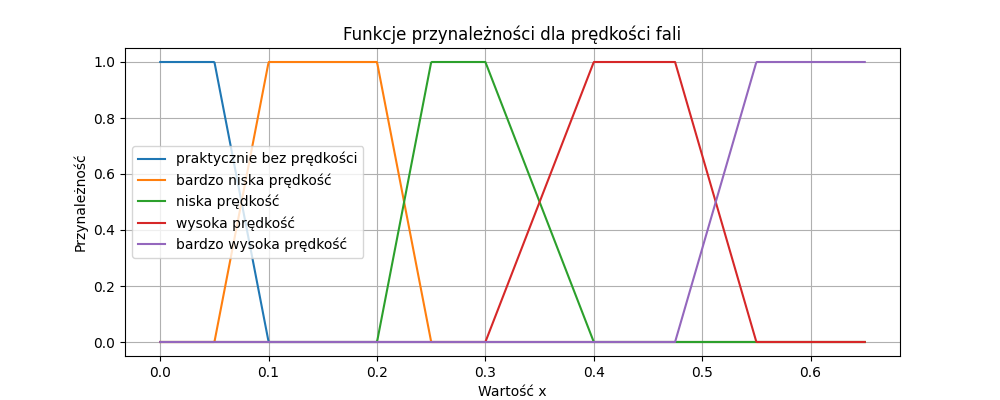
\includegraphics[width=0.5\textwidth]{ksr/projekt_2_fuzzy/assets/wave_speed.png}
\label{fig:epsilon_bat}
\end{figure}

%===================================================================================================
\subsubsection{Głębokość dna}

\noindent Zmienna opisująca, na jakiej głębokości znajduje się dno w miejscu robienia danego pomiaru, głębokość ta opisana została w metrach [m]. Etykiety wraz z funkcjami przynależności opisane zostały poniżej.

\begin{equation*}
\begin{minipage}{0.5\textwidth}
\centering
$\text{\scalebox{0.5}{głębokość przypowierzchniowa}}(x) =
\scalebox{0.5}{$
\begin{cases}
1 & \text{dla } x \leq 4 \\
\frac{10 - x}{6} & \text{dla } 4 < x \leq 10 \\
0 & \text{w przeciwnym przypadku}
\end{cases}
$}$
\end{minipage}%
\begin{minipage}{0.5\textwidth}
\centering
$\text{\scalebox{0.5}{płytko}}(x) =
\scalebox{0.5}{$
\begin{cases}
\frac{x - 6}{4} & \text{dla } 6 < x \leq 10 \\
1 & \text{dla } 10 < x \leq 14 \\
\frac{16 - x}{2} & \text{dla } 14 < x \leq 16 \\
0 & \text{w przeciwnym przypadku}
\end{cases}
$}$
\end{minipage}
\end{equation*}
\begin{equation*}
\begin{minipage}{0.5\textwidth}
\centering
$\text{\scalebox{0.5}{umiarkowanie głęboko}}(x) =
\scalebox{0.5}{$
\begin{cases}
\frac{x - 14}{4} & \text{dla } 14 < x \leq 18 \\
1 & \text{dla } 18 < x \leq 21 \\
\frac{28 - x}{7} & \text{dla } 21 < x \leq 28 \\
0 & \text{w przeciwnym przypadku}
\end{cases}
$}$
\end{minipage}%
\begin{minipage}{0.5\textwidth}
\centering
$\text{\scalebox{0.5}{głęboko}}(x) =
\scalebox{0.5}{$
\begin{cases}
\frac{x - 21}{8} & \text{dla } 21 < x \leq 29 \\
1 & \text{dla } 29 < x \leq 32 \\
\frac{34 - x}{2} & \text{dla } 32 < x \leq 34 \\
0 & \text{w przeciwnym przypadku}
\end{cases}
$}$
\end{minipage}
\end{equation*}
\begin{equation*}
\text{\scalebox{0.5}{profundalnie głęboko}}(x) =
\scalebox{0.5}{$
\begin{cases}
0 & \text{dla } x \leq 32 \\
\frac{x - 32}{2} & \text{dla } 32 < x \leq 34 \\
1 & \text{w przeciwnym przypadku}
\end{cases}
$}
\end{equation*}

\begin{figure}[H]
\centering
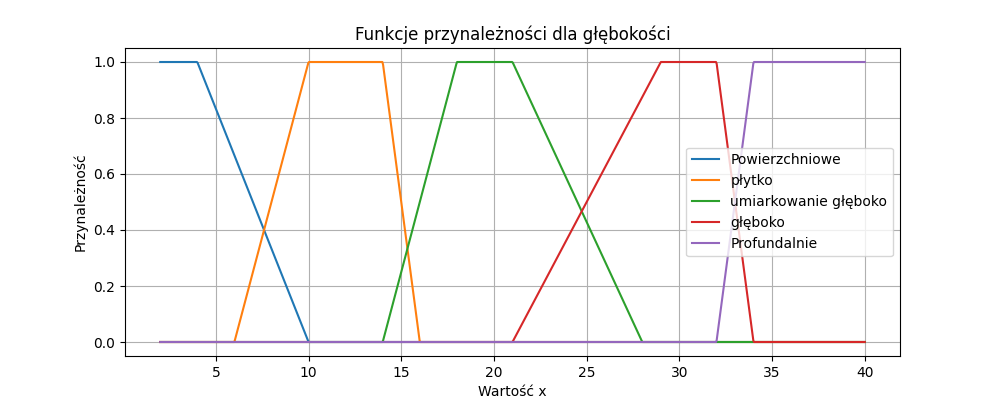
\includegraphics[width=0.5\textwidth]{ksr/projekt_2_fuzzy/assets/depth.png}
\label{fig:epsilon_bat}
\end{figure}

%===================================================================================================
\subsubsection{wysokość fal}

\noindent Wysokość fal to zmienna lingwistyczna mówiąca o tym, jak wysokie fale zostały zarejestrowane w momencie robienia pomiaru. Zmierzona wysokość ta opisana została w jednostkach si, czyli metrach [m]. Dokładny opis o tym, jak mierzy się wspomnianą wysokość opisana została w prezentacji \cite{waves}.

\begin{equation*}
\begin{minipage}{0.5\textwidth}
\centering
$\text{\scalebox{0.5}{spokojne morze}}(x) =
\scalebox{0.5}{$
\begin{cases}
1 & \text{dla } x \leq 0.5 \\
\frac{0.7 - x}{0.2} & \text{dla } 0.5 < x \leq 0.7 \\
0 & \text{w przeciwnym przypadku}
\end{cases}
$}$
\end{minipage}%
\begin{minipage}{0.5\textwidth}
\centering
$\text{\scalebox{0.5}{niewielkie fale}}(x) =
\scalebox{0.5}{$
\begin{cases}
\frac{x - 0.5}{0.7} & \text{dla } 0.5 < x \leq 1.2 \\
1 & \text{dla } 1.2 < x \leq 1.8 \\
\frac{2 - x}{0.2} & \text{dla } 1.8 < x \leq 2 \\
0 & \text{w przeciwnym przypadku}
\end{cases}
$}$
\end{minipage}
\end{equation*}
\begin{equation*}
\begin{minipage}{0.5\textwidth}
\centering
$\text{\scalebox{0.5}{średnie fale}}(x) =
\scalebox{0.5}{$
\begin{cases}
\frac{x - 1.8}{0.7} & \text{dla } 1.8 < x < 2.5 \\
1 & \text{dla } x = 2.5 \\
\frac{2.7 - x}{0.2} & \text{dla } 2.5 < x \leq 2.7 \\
0 & \text{w przeciwnym przypadku}
\end{cases}
$}$
\end{minipage}%
\begin{minipage}{0.5\textwidth}
\centering
$\text{\scalebox{0.5}{wysokie fale}}(x) =
\scalebox{0.5}{$
\begin{cases}
0 & \text{dla } x \leq 2.6 \\
\frac{x - 2.6}{0.1} & \text{dla } 2.6 < x \leq 2.7 \\
1 & \text{w przeciwnym przypadku}
\end{cases}
$}$
\end{minipage}
\end{equation*}

\begin{figure}[H]
\centering
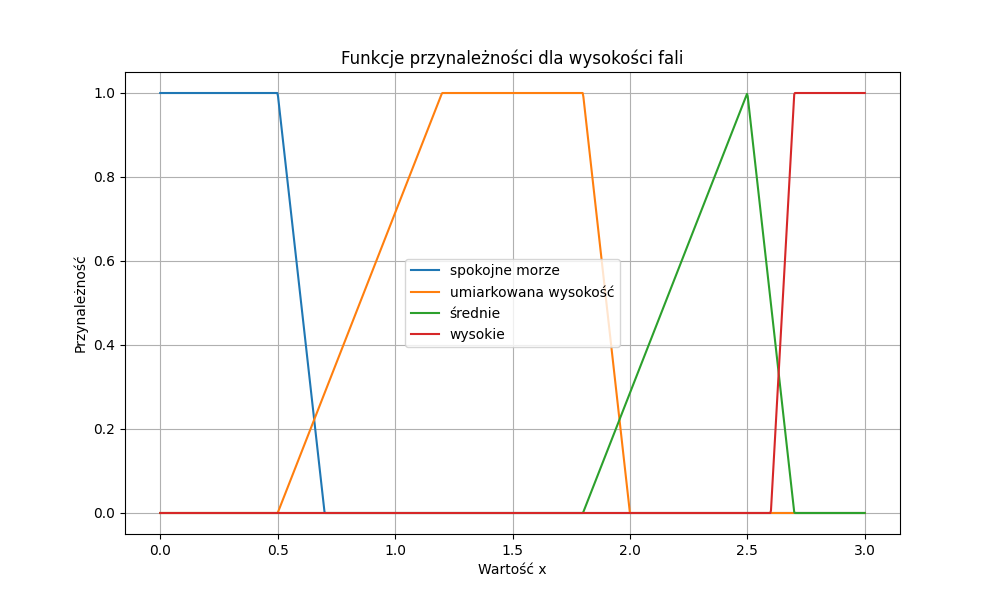
\includegraphics[width=0.5\textwidth]{ksr/projekt_2_fuzzy/assets/wave_hight.png}
\label{fig:epsilon_bat}
\end{figure}

%===================================================================================================
\subsubsection{Kierunek fal}

\noindent Kierunek fal mierzony mówi o tym, w którą stronę skierowane były fale w momencie robienia pomiaru. Wartość ta mierzona była w stopniach, jednakże dla ułatwienia analizy etykiety wybrane dla tej zmiennej zapisane zostały jako kierunki świata.

\begin{equation*}
\begin{minipage}{0.5\textwidth}
\centering
$\text{\scalebox{0.5}{północ}}(x) =
\scalebox{0.5}{$
\begin{cases}
1 & \text{dla } x \leq 0 \\
\frac{32.5 - x}{32.5} & \text{dla } 0 < x \leq 32.5 \\
\frac{x - 327.5}{32.5} & \text{dla } 327.5 < x \leq 360 \\
1 & \text{dla } x \geq 360 \\
0 & \text{w przeciwnym przypadku}
\end{cases}
$}$
\end{minipage}%
\begin{minipage}{0.5\textwidth}
\centering
$\text{\scalebox{0.5}{północny-wschód}}(x) =
\scalebox{0.5}{$
\begin{cases}
\frac{x - 12.5}{32.5} & \text{dla } 12.5 < x \leq 45 \\
1 & \text{dla } x = 45 \\
\frac{77.5 - x}{32.5} & \text{dla } 45 < x \leq 77.5 \\
0 & \text{w przeciwnym przypadku}
\end{cases}
$}$
\end{minipage}
\end{equation*}
\begin{equation*}
\begin{minipage}{0.5\textwidth}
\centering
$\text{\scalebox{0.5}{wschód}}(x) =
\scalebox{0.5}{$
\begin{cases}
\frac{x - 57.5}{32.5} & \text{dla } 57.5 < x \leq 90 \\
1 & \text{dla } x = 90 \\
\frac{122.5 - x}{32.5} & \text{dla } 90 < x \leq 122.5 \\
0 & \text{w przeciwnym przypadku}
\end{cases}
$}$
\end{minipage}%
\begin{minipage}{0.5\textwidth}
\centering
$\text{\scalebox{0.5}{południowy-wschód}}(x) =
\scalebox{0.5}{$
\begin{cases}
\frac{x - 102.5}{32.5} & \text{dla } 102.5 < x \leq 135 \\
1 & \text{dla } x = 135 \\
\frac{167.5 - x}{32.5} & \text{dla } 135 < x \leq 167.5 \\
0 & \text{w przeciwnym przypadku}
\end{cases}
$}$
\end{minipage}
\end{equation*}
\begin{equation*}
\begin{minipage}{0.5\textwidth}
\centering
$\text{\scalebox{0.5}{południe}}(x) =
\scalebox{0.5}{$
\begin{cases}
\frac{x - 147.5}{32.5} & \text{dla } 147.5 < x < 180 \\
1 & \text{dla } x = 180 \\
\frac{212.5 - x}{32.5} & \text{dla } 180 < x \leq 212.5 \\
0 & \text{w przeciwnym przypadku}
\end{cases}
$}$
\end{minipage}%
\begin{minipage}{0.5\textwidth}
\centering
$\text{\scalebox{0.5}{południowy-zachód}}(x) =
\scalebox{0.5}{$
\begin{cases}
\frac{x - 192.5}{32.5} & \text{dla } 192.5 < x \leq 225 \\
1 & \text{dla } x = 225 \\
\frac{257.5 - x}{32.5} & \text{dla } 225 < x \leq 257.5 \\
0 & \text{w przeciwnym przypadku}
\end{cases}
$}$
\end{minipage}
\end{equation*}
\begin{equation*}
\begin{minipage}{0.5\textwidth}
\centering
$\text{\scalebox{0.5}{zachód}}(x) =
\scalebox{0.5}{$
\begin{cases}
\frac{x - 237.5}{32.5} & \text{dla } 237.5 < x \leq 270 \\
1 & \text{dla } x = 270 \\
\frac{302.5 - x}{32.5} & \text{dla } 270 < x \leq 302.5 \\
0 & \text{w przeciwnym przypadku}
\end{cases}
$}$
\end{minipage}%
\begin{minipage}{0.5\textwidth}
\centering
$\text{\scalebox{0.5}{północny-zachód}}(x) =
\scalebox{0.5}{$
\begin{cases}
\frac{x - 282.5}{32.5} & \text{dla } 282.5 < x \leq 315 \\
1 & \text{dla } x = 315 \\
\frac{347.5 - x}{32.5} & \text{dla } 315 < x \leq 347.5 \\
0 & \text{w przeciwnym przypadku}
\end{cases}
$}$
\end{minipage}
\end{equation*}


\begin{figure}[H]
\centering
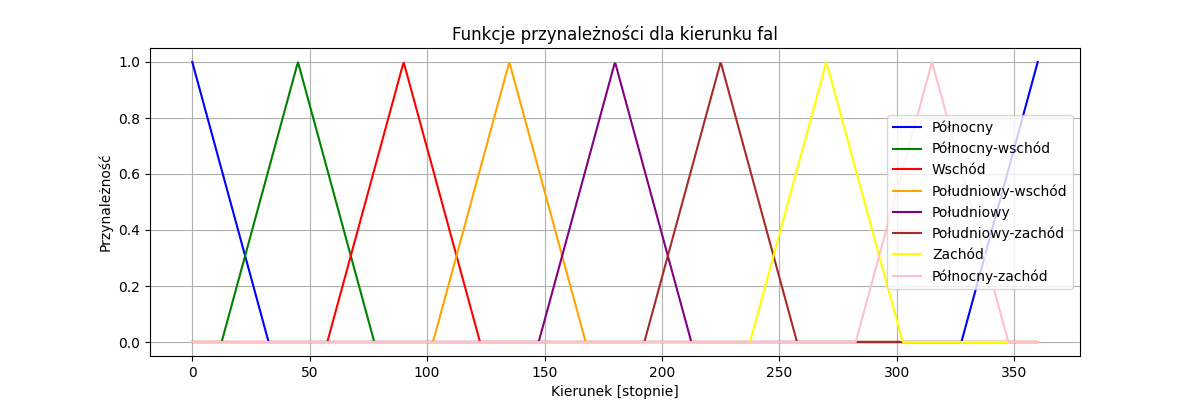
\includegraphics[width=0.6\textwidth]{ksr/projekt_2_fuzzy/assets/wave_direction.png}
\label{fig:epsilon_bat}
\end{figure}

%===================================================================================================
\subsubsection{Częstotliwość fal}

\noindent Zmienna lingwistyczna opisująca częstotliwość tworzenia się fal opisana została przy pomocy etykiet utworzonych na podstawie dokumentu \cite{waves}, niewielka ilość etykiet utworzonych dla tej zmiennej spowodowana jest niewielkim przedziałem częstotliwości tworzenia się fal dla badanego obszaru.

\begin{equation*}
\text{\scalebox{0.5}{zmarszczki}}(x) = \scalebox{0.5}{$\exp\left(-\frac{{(x - 0.5)^2}}{{2 \cdot 0.5^2}}\right)$}
\end{equation*}
\begin{equation*}
\text{\scalebox{0.5}{rzadkie fale wiatrowe}}(x) = \scalebox{0.5}{$\exp\left(-\frac{{(x - 2.6)^2}}{{2 \cdot 0.6^2}}\right)$}
\end{equation*}
\begin{equation*}
\text{\scalebox{0.5}{fale wiatrowe}}(x) = \scalebox{0.5}{$\exp\left(-\frac{{(x - 5)^2}}{{2 \cdot 0.75^2}}\right)$}
\end{equation*}

\begin{figure}[H]
\centering
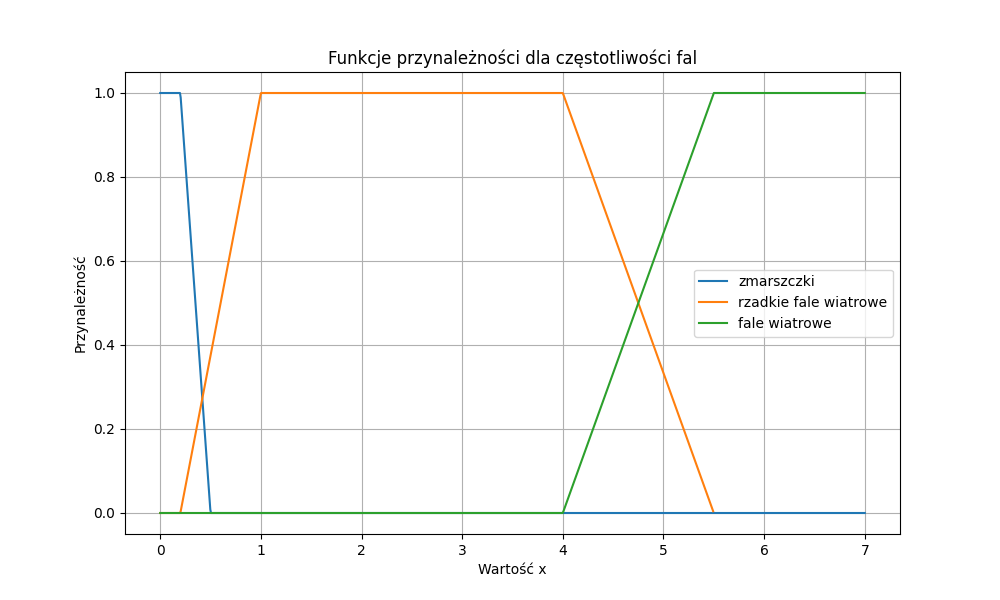
\includegraphics[width=0.6\textwidth]{ksr/projekt_2_fuzzy/assets/wave_frequency.png}
\label{fig:epsilon_bat}
\end{figure}

\subsection{Kwantyfikatory lingwistyczne}

\noindent W ramach projektu opisano kwantyfikatory lingwistyczne, nadając im etykiety oraz prezentując wykresy funkcji przynależności, oraz wzory analityczne. Kwantyfikatory rozmyte względne i absolutne są narzędziami w logice rozmytej służącymi do opisu stopnia przynależności elementów do zbiorów rozmytych. Kwantyfikatory względne odnoszą się do relacji między zbiorami, podczas gdy kwantyfikatory absolutne opisują stopień przynależności wszystkich elementów do konkretnego zbioru rozmytego.\\

\subsubsection{Kwantyfikatory rozmyte względne}

\begin{equation*}
\begin{minipage}{0.5\textwidth}
\centering
\text{\scalebox{0.5}{little}}(x) = \scalebox{0.5}{$
\begin{cases}
1 & \text{dla } x \leq 0.1 \\
\frac{0.3 - x}{0.2} & \text{dla } 0.1 < x \leq 0.3 \\
0 & \text{w przeciwnym przypadku}
\end{cases}
$}
\end{minipage}%
\begin{minipage}{0.5\textwidth}
\centering
\text{\scalebox{0.5}{around\_1\_3}}(x) = \scalebox{0.5}{$
\begin{cases}
0 & \text{dla } x \leq 0.2 \\
10(x - 0.2) & \text{dla } 0.2 < x \leq 0.3 \\
1 & \text{dla } 0.3 < x \leq 0.36 \\
1 - 10(x - 0.36) & \text{dla } 0.36 < x \leq 0.46 \\
0 & \text{w przeciwnym przypadku}
\end{cases}
$}
\end{minipage}
\end{equation*}
\begin{equation*}
\begin{minipage}{0.5\textwidth}
\centering
\text{\scalebox{0.5}{almost\_half}}(x) = \scalebox{0.5}{$
\begin{cases}
0 & \text{dla } x \leq 0.4 \\
14(x - 0.4) & \text{dla } 0.4 < x \leq 0.47 \\
1 & \text{dla } 0.47 < x \leq 0.53 \\
1 - 15(x - 0.53) & \text{dla } 0.53 < x \leq 0.6 \\
0 & \text{w przeciwnym przypadku}
\end{cases}
$}
\end{minipage}%
\begin{minipage}{0.5\textwidth}
\centering
\text{\scalebox{0.5}{around\_2\_3}}(x) = \scalebox{0.5}{$
\begin{cases}
0 & \text{dla } x \leq 0.53 \\
10(x - 0.53) & \text{dla } 0.53 < x \leq 0.63 \\
1 & \text{dla } 0.63 < x \leq 0.7 \\
1 - 10(x - 0.7) & \text{dla } 0.7 < x \leq 0.8 \\
0 & \text{w przeciwnym przypadku}
\end{cases}
$}
\end{minipage}
\end{equation*}
\begin{equation*}
\begin{minipage}{0.5\textwidth}
\centering
\text{\scalebox{0.5}{almost\_all}}(x) = \scalebox{0.5}{$
\begin{cases}
0 & \text{dla } x \leq 0.7 \\
\frac{x - 0.7}{0.2} & \text{dla } 0.7 < x \leq 0.9 \\
1 & \text{w przeciwnym przypadku}
\end{cases}
$}
\end{minipage}
\end{equation*}

\subsubsection{Kwantyfikatory rozmyte absolutne}

\[
\begin{minipage}{0.5\textwidth}
\centering
\text{\scalebox{0.5}{mniej niż 10\%}}(x) = \scalebox{0.5}{$
\begin{cases}
1 & \text{if } x \leq 0.1 \\
0 & \text{otherwise}
\end{cases}
$}
\end{minipage}%
\begin{minipage}{0.5\textwidth}
\centering
\text{\scalebox{0.5}{około 20\%}}(x) = \scalebox{0.5}{$
\begin{cases}
\frac{x - 0.1}{0.1} & \text{if } 0.1 < x < 0.2 \\
1 & \text{if } x = 0.2 \\
\frac{0.3 - x}{0.1} & \text{if } 0.2 < x \leq 0.3 \\
0 & \text{otherwise}
\end{cases}
$}
\end{minipage}
\]
\[
\begin{minipage}{0.5\textwidth}
\centering
\text{\scalebox{0.5}{około 30\%}}(x) = \scalebox{0.5}{$
\begin{cases}
\frac{x - 0.2}{0.1} & \text{if } 0.2 < x \leq 0.3 \\
1 & \text{if } x = 0.3 \\
\frac{0.4 - x}{0.1} & \text{if } 0.3 < x \leq 0.4 \\
0 & \text{otherwise}
\end{cases}
$}
\end{minipage}%
\begin{minipage}{0.5\textwidth}
\centering
\text{\scalebox{0.5}{około 40\%}}(x) = \scalebox{0.5}{$
\begin{cases}
\frac{x - 0.3}{0.1} & \text{if } 0.3 < x \leq 0.4 \\
1 & \text{if } x = 0.4 \\
\frac{0.5 - x}{0.1} & \text{if } 0.4 < x \leq 0.5 \\
0 & \text{otherwise}
\end{cases}
$}
\end{minipage}
\]
\[
\begin{minipage}{0.5\textwidth}
\centering
\text{\scalebox{0.5}{około 50\%}}(x) = \scalebox{0.5}{$
\begin{cases}
\frac{x - 0.4}{0.1} & \text{if } 0.4 < x \leq 0.5 \\
1 & \text{if } x = 0.5 \\
\frac{0.6 - x}{0.1} & \text{if } 0.5 < x \leq 0.6 \\
0 & \text{otherwise}
\end{cases}
$}
\end{minipage}%
\begin{minipage}{0.5\textwidth}
\centering
\text{\scalebox{0.5}{około 60\%}}(x) = \scalebox{0.5}{$
\begin{cases}
\frac{x - 0.5}{0.1} & \text{if } 0.5 < x \leq 0.6 \\
1 & \text{if } x = 0.6 \\
\frac{0.7 - x}{0.1} & \text{if } 0.6 < x \leq 0.7 \\
0 & \text{otherwise}
\end{cases}
$}
\end{minipage}
\]
\[
\begin{minipage}{0.5\textwidth}
\centering
\text{\scalebox{0.5}{około 70\%}}(x) = \scalebox{0.5}{$
\begin{cases}
\frac{x - 0.6}{0.1} & \text{if } 0.6 < x \leq 0.7 \\
1 & \text{if } x = 0.7 \\
\frac{0.8 - x}{0.1} & \text{if } 0.7 < x \leq 0.8 \\
0 & \text{otherwise}
\end{cases}
$}
\end{minipage}%
\begin{minipage}{0.5\textwidth}
\centering
\text{\scalebox{0.5}{około 80\%}}(x) = \scalebox{0.5}{$
\begin{cases}
\frac{x - 0.7}{0.1} & \text{if } 0.7 < x \leq 0.8 \\
1 & \text{if } x = 0.8 \\
\frac{0.9 - x}{0.1} & \text{if } 0.8 < x \leq 0.9 \\
0 & \text{otherwise}
\end{cases}
$}
\end{minipage}
\]
\[
\begin{minipage}{0.5\textwidth}
\centering
\text{\scalebox{0.5}{więcej niż 90\%}}(x) = \scalebox{0.5}{$
\begin{cases}
0 & \text{if } x \leq 0.9 \\
1 & \text{otherwise}
\end{cases}
$}
\end{minipage}
\]


\subsubsection{wykresy wybranych kwalifikatorów lingwistycznych}


\begin{table}[H]
\centering
\begin{tabular}{cc}
    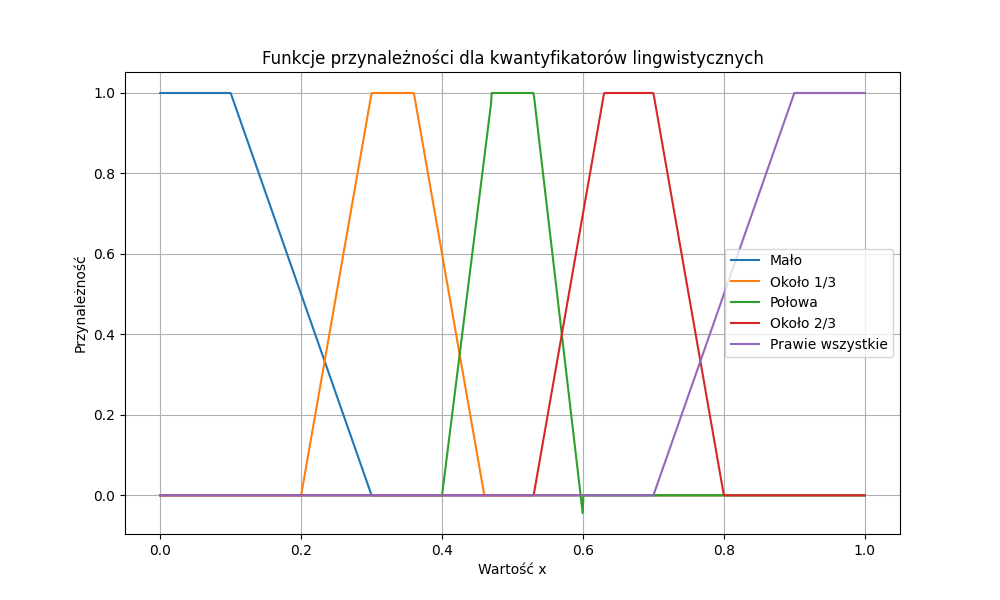
\includegraphics[width=0.5\textwidth]{ksr/projekt_2_fuzzy/assets/qualifiers.png} &
    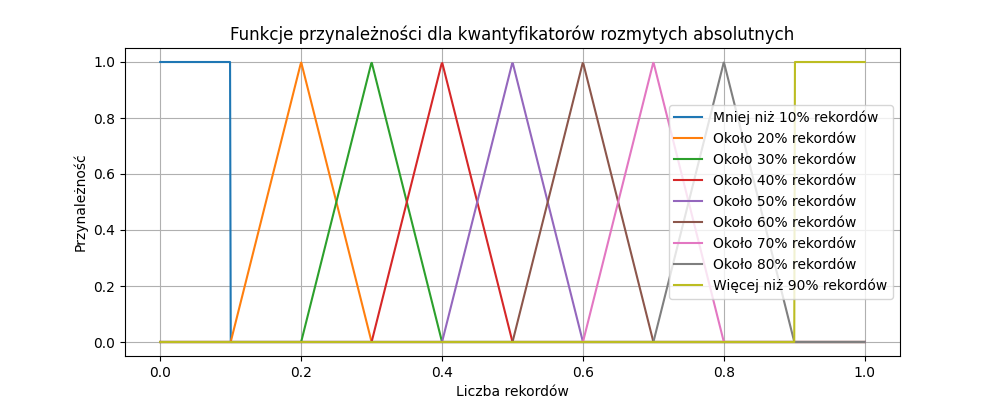
\includegraphics[width=0.5\textwidth]{ksr/projekt_2_fuzzy/assets/qualifiers2.png} \\
     \\
\end{tabular}
\label{fig:two_images}
\end{table}


Opisy zostały przygotowane z uwzględnieniem literatury dotyczącej lingwistyki rozmytej oraz jej zastosowań.




%=======================================================================================

\section{Narzędzia obliczeniowe: wybór/implementacja. Diagram UML pakietu
obliczeń rozmytych i~generatora podsumowań. Instrukcja użytkownika}


\subsection{Opis pakietu obliczeń rozmytych - fuzzyLib}

\noindent W celu zaspokojenia wymagań zadania utworzony został pakiet przeznaczony do obsługi logiki aplikacji. Poniżej zaprezentowany został diagram UML przedstawiający strukturę pakietu oraz jego pakietów pochodnych.

\begin{figure}[H]
\centering
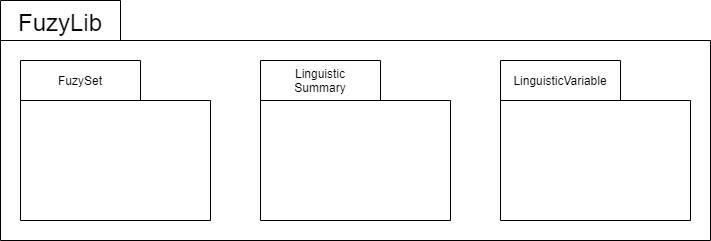
\includegraphics[width=0.6\textwidth]{ksr/projekt_2_fuzzy/assetsUml/packets.png}
\caption{pakiet fuzzyLib wraz z jego podpakietami}
\label{fig:epsilon_bat}
\end{figure}

\noindent Warto tutaj zaznaczyć że przedstawione w tej sekcji UML'e nie zawierają metod pomocniczych (setery i getery), które zaimplementowe są domyślnie.

\subsubsection{pakiet FuzzySet}

\noindent Pakiet definiujący interfejsy i implementacje funkcji przynależności, które są elementarnymi składnikami zbiorów rozmytych. Zawiera klasy i narzędzia służące do tworzenia, analizy i manipulacji tymi funkcjami. Dodatkowo klasa abstrakcyjna FuzzySet zapewnia operacje możliwe do przeprowadzenia na zbiorach rozmytych

\begin{itemize}
    \item[FuzzySet:] Klasa abstrakcyjna po której dziedziczą wszystkie pozostałe klasy reprezentujące zbiory rozmyte oraz ich funkcje przynależności, udostępnia operacje możliwe do wykonania na zbiorach rozmytych (dopełnienie, liczba kardynalna czy alfa cut).
    \item[FuzzySetFactoryConsts:] Zawiera stałe reprezentujące różne typy funkcji przynależności, takie jak TRIANGULAR, TRAPEZOIDAL i GAUSSIAN.
    \item[FuzzySetFactory:] Fabryka do tworzenia różnych typów funkcji przynależności na podstawie podanego typu oraz parametrów.
    Wykorzystuje wyrażenie switch do dynamicznego tworzenia odpowiednich instancji klas na podstawie podanego typu.
    \item[TrapezoidalFuzzySet:] Reprezentuje funkcję przynależności trapezoidalnej w ramach zbioru rozmytego.
    \item[TriangularFuzzySet:] Reprezentuje funkcję przynależności trójkątną w ramach zbioru rozmytego.
    \item[GaussianFuzzySet:] Reprezentuje funkcję przynależności Gaussa w ramach zbioru rozmytego.
\end{itemize}

\begin{figure}[H]
\centering
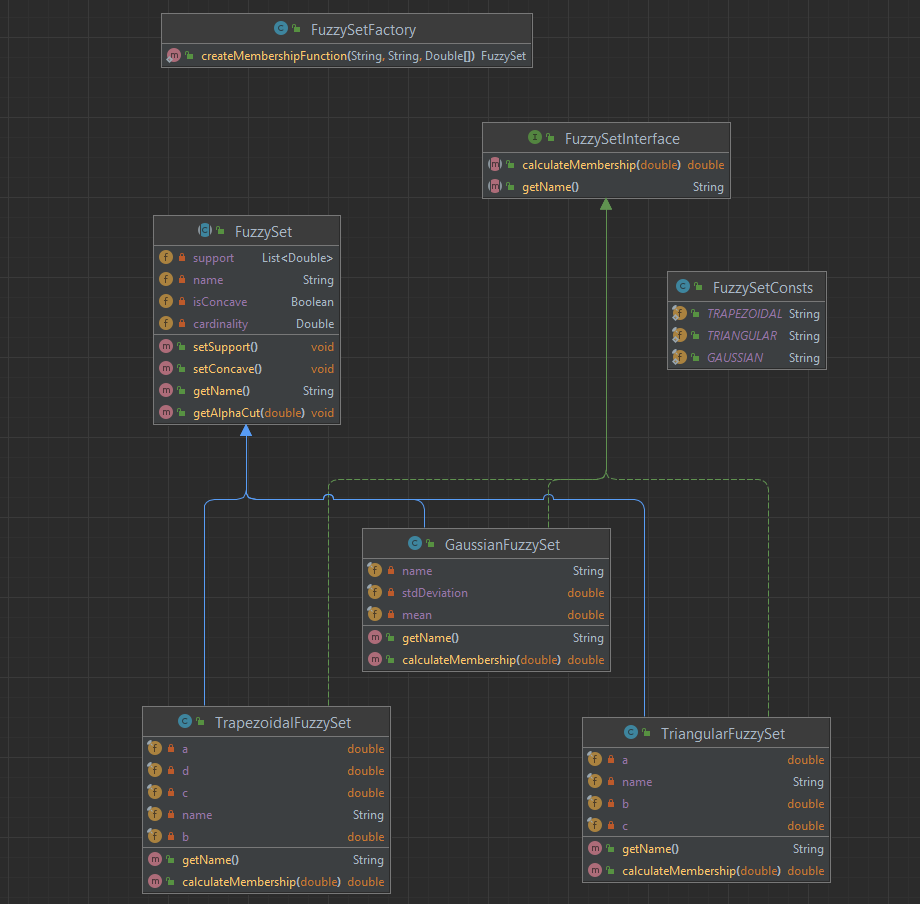
\includegraphics[width=0.6\textwidth]{ksr/projekt_2_fuzzy/assetsUml/FuzzySet.png}
\caption{Pakiet MembershipFunction}
\label{fig:epsilon_bat}
\end{figure}

\subsubsection{Pakiet LinguisticSummary}

\noindent Pakiet zajmujący się generowaniem podsumowań lingwistycznych, czyli formułowania wniosków na podstawie zbiorów rozmytych. Zawiera klasy i narzędzia do tworzenia podsumowań lingwistycznych różnych stopni złożoności, w oparciu o zbiory rozmyte jako elementy wnioskowania.

\begin{itemize}
    \item[Label:] Klasa pomocnicza służąca do obsługi kwalifikatorów oraz kwantyfikatorów, przechowuje nazwę funkcji przynależności oraz zmienną lingwistyczną. Dzięki tem jesteśmy wstanie określić przestrzeń rozważań oraz posługiwać się odpowiednią funkcją podczas tworzenia podsumowań.
    \item[LinguisticSummary:]  Jest to klasa abstrakcyjna reprezentująca podsumowanie lingwistyczne. Posiada pola takie jak qualifier (kwalifikator), summarizer (sumatory), truthChecker (obiekt sprawdzający prawdziwość) i quantifier (kwantyfikator). Udostępnia metody do tworzenia podsumowań lingwistycznych. Uwaga, podmiot pobierany jest bezpośrednio z bazy danych wewnątrz "createLinguisticSummary".
    \item[TruthChecker:] Jest to klasa służąca do sprawdzania stopnia prawdziwości podsumowań lingwistycznych. Jest zaimplementowana jako Singleton, aby zapewnić tylko jedną instancję tej klasy w aplikacji.
\end{itemize}

\begin{figure}[H]
\centering
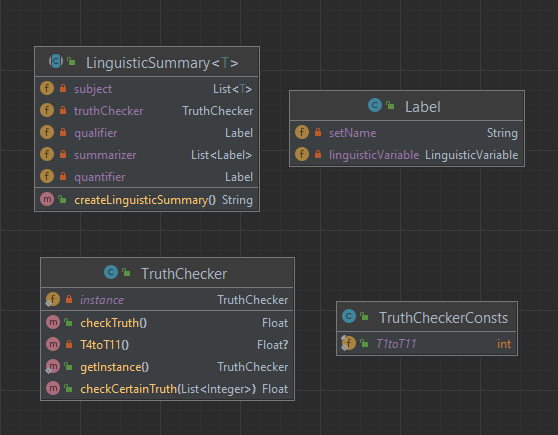
\includegraphics[width=0.6\textwidth]{ksr/projekt_2_fuzzy/assetsUml/LinguisticSummary.png}
\caption{Pakiet LinguisticSummary}
\label{fig:epsilon_bat}
\end{figure}

\noindent Tu warto zaznaczyć, że klasy TruthChecker oraz TrutchCheckerConsts zawierają tylko poglądową ilość pul związanych z funkcjami jakości podsumowania lingwistycznego, ich docelowa ilość to 11 (od T1 do T11).

\subsubsection{Pakiet LinguisticVariable}

\noindent Pakiet odpowiedzialny za reprezentację i zarządzanie zbiorami rozmytymi. Zawiera klasy i narzędzia do definiowania, manipulowania i analizowania zbiorów rozmytych \cite{niewiadomski19}, w tym klasy reprezentujące same zbiory rozmyte oraz fabrykę umożliwiającą ich tworzenie.

\begin{itemize}
    \item[LinguisticVariable:] Jest to abstrakcyjna klasa reprezentująca zmienną lingwistyczną. Zawiera pola takie jak nazwa, lista funkcji przynależności. Udostępnia metody do dodawania i usuwania funkcji przynależności. Celem tej klasy jest reprezentowanie takich wartości jak na przykład kwalifikator bądź sumaryzator.
    \item[Pakiet Assets:] mimo że nie należy bezpośrednio do pakietu linguisticVariable to zawiera on implementacje zmiennych lingwistycznych dziedziczących po klasie abstrakcyjnej LinguisticVariable, znajduje się on poza wspomnianym pakietem ponieważ obsługuje on również wczytywanie wartości z plików konfiguracyjnych.
\end{itemize}

\begin{figure}[H]
\centering
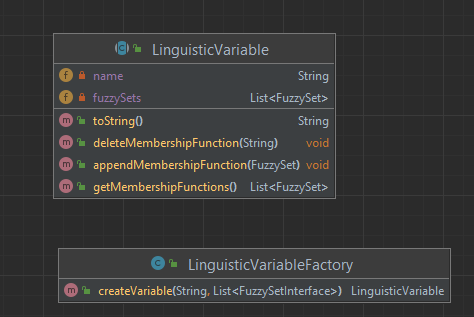
\includegraphics[width=0.6\textwidth]{ksr/projekt_2_fuzzy/assetsUml/LinguisticVariable.png}
\caption{Pakiet FuzzySet}
\label{fig:epsilon_bat}
\end{figure}

\subsection{Interfejs użytkownika}

\noindent Aplikacja posiada relatywnie intuicyjny interfejs użytkownika składający się z 2 paneli, pierwszy z nich służy do generowania podsumowań lingwistycznych, drugi to tak zwany interfejs użytkownika zaawansowanego pozwalający na tworzenie i dodawanie funkcji przynależności do danych zmiennych lingwistycznych. Cały front naszego programu realizowany jest przez pakiet "Gui" \\

\subsubsection{Panel główny}

\noindent Panel główny aplikacji pozwala na wybranie z listy dostępnych obiektów kwantyfikatora, kwalifikatora oraz do 3 sumatyzatorów, po zatwierdzeniu parametrów wynik wyświetlony zostanie po lewej stronie ekranu.

\begin{figure}[H]
\centering
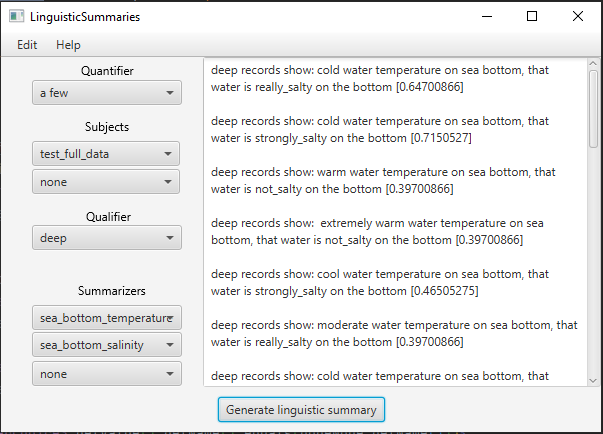
\includegraphics[width=0.6\textwidth]{ksr/projekt_2_fuzzy/assetsGui/mainView.png}
\caption{główny ekran aplikacji}
\label{fig:epsilon_bat}
\end{figure}

\subsubsection{Panel użytkownika zaawansowanego}

\noindent Wejście do panelu użytkownika zaawansowanego odbywa się poprzez panel Edit-> enter edit mode, w ten sam sposób można wspomniany panel opuścić Edit -> exit edit mode.

\begin{figure}[H]
\centering
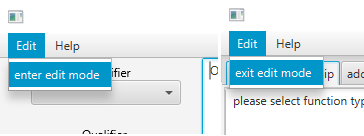
\includegraphics[width=0.6\textwidth]{ksr/projekt_2_fuzzy/assetsGui/edit_exit_editMode.png}
\caption{przełączanie się między panelem użytkownika zaawansowanego a panelem głównym}
\label{fig:epsilon_bat}
\end{figure}

\begin{figure}[H]
  \begin{minipage}[b]{0.3\linewidth}
    \centering
    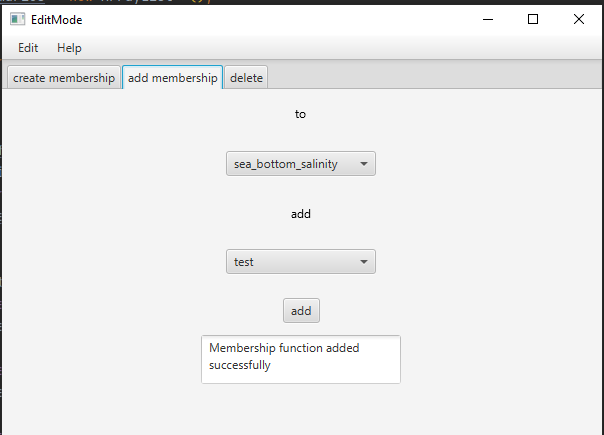
\includegraphics[width=\linewidth]{ksr/projekt_2_fuzzy/assetsGui/editMode.png}
    \caption{ekran tworzenia funkcji przynależności}
  \end{minipage}
  \hfill
  \begin{minipage}[b]{0.3\linewidth}
    \centering
    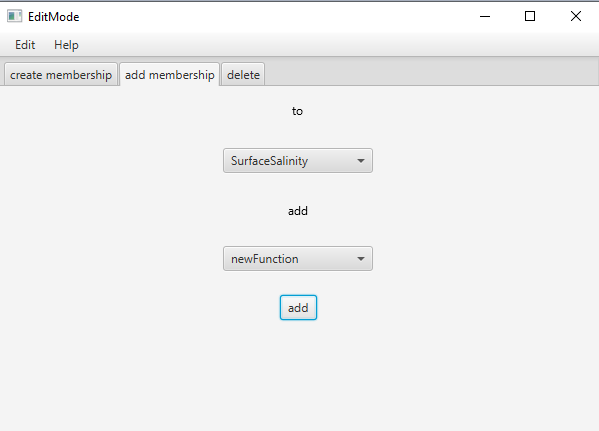
\includegraphics[width=\linewidth]{ksr/projekt_2_fuzzy/assetsGui/EditModeAdd.png}
    \caption{ekran dodawania funkcji przynależności do zmiennej lingwistycznej}
  \end{minipage}
  \hfill
  \begin{minipage}[b]{0.3\linewidth}
    \centering
    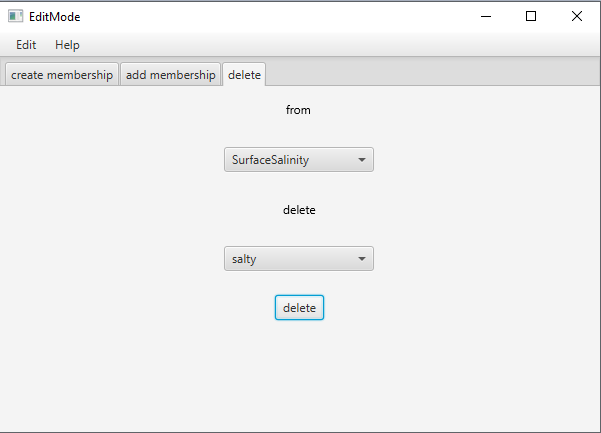
\includegraphics[width=\linewidth]{ksr/projekt_2_fuzzy/assetsGui/editModeDelete.png}
    \caption{ekran usuwania funkcji przynależności ze zmiennej lingwistycznej}
  \end{minipage}
\end{figure}

\noindent Utworzenie nowej funkcji przynależności odbywa się poprzez wybranie kształtu funkcji (trójkątna, trapezoidalna oraz gausowska) oraz wprowadzenie odpowiednich parametrów. W celu dodania/usunięcia funkcji ze zmiennej lingwistycznej należy skorzystać z odpowiednich paneli.


\subsection{JRE}

\noindent Aby uruchomić naszą aplikację, użytkownik musi mieć zainstalowane środowisko uruchomieniowe Java (Java Runtime Environment, JRE). Aplikacja została przetestowana i działa z najnowszą wersją JRE LTS (Long-Term Support), co zapewnia stabilność i długoterminowe wsparcie.

\noindent Aplikacja do poprawnego działania wymaga dostępu do relacyjnej bazy danych. Stworzona została z myślą o użyciu PostgreSQL 13. Użytkownik musi zainstalować i skonfigurować bazę danych oraz dostarczyć odpowiednie dane dostępowe. Dodatkowo Aplikacja wykorzystuje biblioteki Java, które są zarządzane przez system budowania Maven. Użytkownik musi mieć zainstalowany Maven w wersji 3.6.3 lub nowszej.

%=======================================================================================

\section{ Jednopodmiotowe podsumowania lingwistyczne. Miary jakości, podsumowanie optymalne}

\subsection{Wstęp do Eksperymentów}

W ramach niniejszej sekcji sprawozdania przeprowadzono serię eksperymentów mających na celu analizę skuteczności różnych rodzajów podsumowań jednopodmiotowych. Eksperymenty te zostały zrealizowane poprzez opracowanie tabel i rankingów podsumowań dla danych atrybutów. W każdym eksperymencie szczegółowo opisano zastosowane miary jakości, a także dokonano oceny jakości podsumowania optymalnego. Należy również wspomnieć że eksperymenty wykonywane były na całej bazie danych to jest 210 tysiącach rekordów.\\

\noindent W trakcie wyznaczania miary jakości wygenerowanych podsumowań lingwistycznych wykorzystaliśmy wszystkie miary możliwe do wykorzystania dla danego przypadku zgodnie z materiałem źrudłowym \cite{niewiadomski19}. Dodatkowo w celu uzyskania wiarygodnych wyników wykorzystane zostały odpowiednie wagi nałożone na poszegulne miary jakości, ich rozkład zaprezentowany został w poniższych tabelach.


\begin{table}[H]
    \centering
\caption{Przyjęte wagi nałożone na miary jakości dla jednopodmiotowych podsumowań lingwistycznych typu pierwszego}
\label{tab:my_label}
    \begin{tabular}{|c|c|c|c|c|c|c|c|c|c|c|c|} \hline 
        miara jakości & T1 & T2 & T3 & T4 & T5 & T6 & T7 & T8 & T9 & T10 & T11\\ \hline 
        przyjęta waga & 1 & 1 & 1 & 1 & 1 & 1 & 1 & 1 & - & - & -\\ \hline
    \end{tabular}
\end{table}

\begin{table}[H]
    \centering
\caption{Przyjęte wagi nałożone na miary jakości dla jednopodmiotowych podsumowań lingwistycznych typu drugiego}
\label{tab:my_label}
    \begin{tabular}{|c|c|c|c|c|c|c|c|c|c|c|c|} \hline 
        miara jakości & T1 & T2 & T3 & T4 & T5 & T6 & T7 & T8 & T9 & T10 & T11\\ \hline 
        przyjęta waga & 1 & 1 & 1 & 1 & 1 & 1 & 1 & 1 & 1 & 1 & 1\\ \hline
    \end{tabular}
\end{table}

\noindent W celu uzyskania miary jakości z przedziału [0-1] wartość ta wyznaczona została poprzez zastosowanie odpowiedniej średniej.

%======================================================================================

\subsection{Eksperyment dla posumowania jednopodmiotowego w formie pierwszej dla maksymalnej ilosci sumaryzatorów}

Do przeprowadzenia poniższego eksperymentu wykorzystane zostały następne wartości sumaryzatorów, oraz kwantyfikatorów:

\begin{itemize}
    \item[sumaryzatory]: sea\_surface\_temperature, significant\_wave\_height, mixed\_layer\_depth.
    \item[kwantyfikator relatywny]: about\_one\_third.
\end{itemize}

\subsubsection{Wyniki eksperymentu}

\noindent W poniższej tabeli w kolumnie zamieszczone zostało 5 najlepszych podsumowań znlaezionych dla aplikacji uruchomionej z wybranymi prarametramy zamieszczonymi powyżej, łączna ilość znalezionych podsumowań wynosi 80. Dodatkowo wyznaczone zostało porównanie różnicy między najlepszym znalezionym rozwiązaniem, nazwanym tutaj podsumowaniem optymalnym.

\begin{longtable}{|p{0.9\linewidth}|c|c|}
\hline
\textbf{Podsumowanie} & \textbf{T} & \textbf{\(\Delta \)T} \\
\hline
about one third records show: moderate water temperature on sea surface, medium height waves, that sea is moderately shallow & 0.55 & 0.0 \\ \hline
about one third records show: moderate water temperature on sea surface, medium height waves, sea is almost on surface level depth & 0.519 & 0.03 \\ \hline
about one third records show: cold water temperature on sea surface, medium height waves, that sea is moderately shallow & 0.511 & 0.039 \\ \hline
about one third records show: cool water temperature on sea surface, medium height waves, that sea is moderately shallow & 0.511 & 0.039 \\ \hline
about one third records show: warm water temperature on sea surface, medium height waves, that sea is moderately shallow & 0.511 & 0.039 \\ \hline
\hline
\end{longtable}

\noindent Średnia wszystkich miar jakości dla uzyskacnyh podsumowań wyniosła: 0.413


%======================================================================================

\subsection{Eksperyment dla posumowania jednopodmiotowego w formie drugiej przy wykorzystaniu maksymalnej dopuszczalnej ilości sumaryzatrorów}

Do przeprowadzenia poniższego eksperymentu wykorzystane zostały te same wartości sumaryzatorów, oraz kwantyfikatorów co w poprzednim eksperymencie, dodatkowo wykorzystany został następujący kwalifikator:

\begin{itemize}
    \item[kwalifikator]: east\_of\_Ireland z przestrzeni zmiennej lingwistycznej longitude.
\end{itemize}

\subsubsection{Wyniki eksperymentu}

\noindent Tak jak zostało to wykonane dla poprzedniej subsekcji poniższej zamieszczone zostało 5 najlepszych podsumowań znlaezionych dla aplikacji uruchomionej z wybranymi prarametramy zamieszczonymi powyżej. Dodatkowo wyznaczone zostało porównanie różnicy między najlepszym znalezionym rozwiązaniem, nazwanym tutaj podsumowaniem optymalnym.

\begin{longtable}{|p{0.9\linewidth}|c|c|}
\hline
\textbf{Podsumowanie} & \textbf{T} & \textbf{\(\Delta \)T} \\
\hline
about one third records having that record was made east of Ireland show: warm water temperature on sea surface, moderately height waves, that sea is moderately shallow & 0.635 & 0.0 \\ \hline
about one third records having that record was made east of Ireland show: warm water temperature on sea surface, medium height waves, that sea is moderately shallow & 0.611 & 0.025 \\ \hline
about one third records having that record was made east fo Ireland show: warm water temperature on sea surface, calm seas, that sea is moderately shallow & 0.604 & 0.031 \\ \hline
about one third records having that record was made east of Ireland show: warm water temperature on sea surface, height waves, that sea is moderately shallow & 0.604 & 0.031 \\ \hline
about one third records having that record was made east of Ireland show: warm water temperature on sea surface, moderately height waves, sea is almost on surface level depth & 0.595 & 0.04 \\ \hline
\hline
\end{longtable}

\noindent Średnia wszystkich miar jakości dla uzyskacnyh podsumowań wyniosła: 0.501

%======================================================================================

\subsection{Wnioski}

\noindent Podczas analizy skuteczności różnych rodzajów podsumowań jednopodmiotowych na całej bazie danych, zauważono, że istnieją pewne kombinacje sumaryzatorów i kwantyfikatorów, które skutkują podsumowaniami optymalnymi o wysokiej jakości. \\

\noindent Wniosek ten sugeruje, że dobór odpowiednich sumaryzatorów, kwantyfikatorów i ewentualnych kwalifikatorów może istotnie wpłynąć na skuteczność podsumowań lingwistycznych, umożliwiając generowanie optymalnych podsumowań o wysokiej jakości. \\

\noindent Dodatkowo, podczas pracy nad wyliczaniem wartości poprawności podsumowania lingwistycznego, zauważono, że niektóre wartości miary T przyjmują skrajne wartości (tj. 0 i 1). W związku z tym, dobrym pomysłem byłoby nałożenie odpowiednich wag na te wartości T, co mogłoby prowadzić do bardziej zrównoważonych i realistycznych wyników. Nałożenie takich wag pozwoliłoby na uwzględnienie stopnia pewności podsumowań, a tym samym zwiększyłoby ich użyteczność i dokładność w praktycznych zastosowaniach.



%=========================================================================================

\section{Wielopodmiotowe podsumowania lingwistyczne i~ich miary jakości}

\noindent Na potrzeby trego eksperymentu zmuszeni zostaliśmy wyostrzyć jeden ze zbiorów rozmytych, po gruntownej analizie zdecydowaliśmy się wyostrzyć zmienną lingwistyczną "latitude" ze względu na jej mniej więcej równy podział pomiędzy wartości. Dzięki tej operacji uzyskaliśmy 3 podmioty:

\begin{itemize}
    \item records\_from\_north
    \item records\_on\_Irland
    \item records\_from\_south
\end{itemize}


\subsection{Wstęp do Eksperymentów}

\noindent W tej sekcji sprawozdania przeprowadzono serię eksperymentów mających na celu analizę skuteczności różnych rodzajów podsumowań wielopodmiotowych. Nasza aplikacja automatycznie generuje wszystkie cztery rodzaje podsumowań, bez możliwości wyboru konkretnego typu. Eksperymenty te zostały zrealizowane poprzez opracowanie tabel i rankingów podsumowań dla danych atrybutów. W każdym eksperymencie szczegółowo opisano zastosowane miary jakości. Eksperymenty były wykonywane na całej bazie danych, obejmującej 210 tysięcy rekordów. \\

\noindent W celu zapewnienia rzetelności wyników, dane dla dwóch podmiotów były przetwarzane i analizowane w kontekście różnych lingwistycznych zmiennych i ich wartości. Proces generowania podsumowań obejmował:

\begin{itemize}
    \item[Generowanie Podsumowań Typu 1]: Analiza porównawcza pomiędzy dwoma podmiotami bez dodatkowych kwalifikatorów, uwzględniająca wyłącznie lingwistyczne zmienne podsumowujące.
    \item[Generowanie Podsumowań Typu 2]: Porównanie pomiędzy podmiotami z uwzględnieniem kwalifikatora, który filtrował dane na podstawie określonego kryterium.
    \item[Generowanie Podsumowań Typu 3]: Porównanie z uwzględnieniem kwalifikatora w odniesieniu do jednego z podmiotów.
    \item[Generowanie Podsumowań Typu 4]: Ocena inkluzji zbiorów rozmytych typu 2, mająca na celu określenie relacji porządkującej pomiędzy danymi podmiotami.
\end{itemize}

\subsubsection{Przyjęte wartości niezbędne do wykonania eksperymentu}

\begin{itemize}
    \item[podmioty]: records\_from\_north, records\_from\_south 
    \item[sumaryzatory]: sea\_surface\_temperature, significant\_wave\_height, mixed\_layer\_depth.
    \item[kwantyfikator relatywny]: about\_one\_third.
    \item[kwalifikator]: east\_of\_Ireland z przestrzeni zmiennej lingwistycznej longitude.
\end{itemize}

\subsubsection{Wyniki eksperymentu}

\noindent Poniższej zamieszczone zostały najlepsze podsumowania dla każdego typu podsumowań lingwistycznych wygenerowanych dla dwuch podmiotów.

\begin{longtable}{|p{0.9\linewidth}|c|}
\hline
\textbf{Podsumowanie} & \textbf{T} \\
\hline
about one third test\_south\_data comparing to test\_north\_data show: moderate water temperature on sea surface, medium height waves, that sea is deep & 0.5 \\
\hline
\end{longtable}

\noindent Średnia wszystkich miar jakości dla uzyskanych podsumowań wyniosła: 0.458

\begin{longtable}{|p{0.9\linewidth}|c|}
\hline
\textbf{Podsumowanie} & \textbf{T} \\
\hline
about one third test\_south\_data comparing to test\_north\_data having that record was made east of Ireland show: moderate water temperature on sea surface, moderately height waves, that sea is moderately shallow & 0.212 \\
\hline
\end{longtable}

\noindent Średnia wszystkich miar jakości dla uzyskanych podsumowań wyniosła: 0.177

\begin{longtable}{|p{0.9\linewidth}|c|}
\hline
\textbf{Podsumowanie} & \textbf{T} \\
\hline
about one third test\_south\_data having that record was made east of Ireland comparing to test\_north\_data show: cool water temperature on sea surface, medium height waves, that sea is deep & 0.788 \\
\hline
\end{longtable}

\noindent Średnia wszystkich miar jakości dla uzyskanych podsumowań wyniosła: 0.722

\begin{longtable}{|p{0.9\linewidth}|c|}
\hline
\textbf{Podsumowanie} & \textbf{T} \\
\hline
more test\_south\_data than test\_north\_data show: warm water temperature on sea surface, medium height waves, that sea is moderately shallow & 0.266 \\
\hline
\end{longtable}

\noindent Średnia wszystkich miar jakości dla uzyskanych podsumowań wyniosła: 0.109

%======================================================================================

\subsection{Wnioski}

\noindent Ponadto, zaobserwowano, że metoda wielopodmiotowych podsumowań lingwistycznych jest szczególnie skuteczna w kontekście analizy porównawczej różnych grup danych. Ta metodologia dostarcza cennych informacji o relacjach między podmiotami, wskazując na potencjalne dominacje cech w poszczególnych grupach. \\

\noindent Ogólnie rzecz biorąc, wielopodmiotowe podsumowania lingwistyczne wykazały swoją skuteczność w generowaniu intuicyjnych i relatywnie wartościowych wniosków, co może mieć zastosowanie w różnych dziedzinach.

%=========================================================================================

\section{Dyskusja, wnioski}



%=========================================================================================

\begin{thebibliography}{99}
 \bibitem{niewiadomski19} A. Niewiadomski, Zbiory rozmyte typu 2. Zastosowania w reprezentowaniu informacji.  Seria „Problemy współczesnej informatyki” pod redakcją L. Rutkowskiego. Akademicka Oficyna Wydawnicza EXIT, Warszawa, 2019.
\bibitem{zadrozny06} S. Zadrożny, Zapytania nieprecyzyjne i lingwistyczne podsumowania baz danych, EXIT, 2006, Warszawa
\bibitem{niewiadomski08} A. Niewiadomski, Methods for the Linguistic Summarization of Data: Applications of Fuzzy Sets and Their Extensions, Akademicka Oficyna Wydawnicza EXIT, Warszawa, 2008.
\bibitem{dataBase} Marine Institute Monthly Model Means: https://data.world/marineinstitute/b2348da6-873f-4ebb-a03c-5280ee2cf025
\bibitem{waves} Mechanizm falowania wod morskich Kryteria podzialu i typy falowania morz
\end{thebibliography}

Literatura zawiera wyłącznie źródła recenzowane i/lub o potwierdzonej wiarygodności,
możliwe do weryfikacji i cytowane w sprawozdaniu.
\end{document}
